\chapter{Results}  %Title of the First Chapter

\ifpdf
    \graphicspath{{Chapter1/Figs/Raster/}{Chapter1/Figs/PDF/}{Chapter1/Figs/}}
\else
    \graphicspath{{Chapter1/Figs/Vector/}{Chapter1/Figs/}}
\fi

\section{Frequency Splittings due to Differential Rotation} %Section - 1.1 
In this treatment we show that while taking very closely spaced multiplets, the isolated multiplet condition breaks down and there is significant cross coupling across modes due to differential rotation alone. Because axis symmetry imposes the $m'=m$ selection rule, the supermatrix $Z_{k'k}$ of perturbation $\dLd$ is a sparse matrix consisting of diagonals and subdiagonal as show in figure (\ref{fig:coup_mat}). As a case study, we choose to investigate the splitting coefficients of the mode $\mode{0}{77}$ as a result of cross coupling with its neighbouring modes which all lie withing an interval of $100\mu Hz$.

\subsection{Splitting with pure rotation}
We plot the split frequencies $\mode{0}{77}$ along with some neighbouring modes to contrast the results obtained from a QDPT and a DPT analysis.

\begin{table}
\begin{center}
\begin{tabular}{|l|c|c|c|c|c|c|c|c|r|}
\hline
$_n\bm{S}_l$ 
& \mode{0}{69}
& \mode{0}{71}  
& \mode{0}{73} 
& \mode{0}{75} 
& \mode{0}{77} 
& \mode{0}{79} 
& \mode{0}{81}  
& \mode{0}{83} 
& \mode{0}{85}
\\ \hline
$\bm{\omega}_{nl}$ 
& \hfill 848.219 
& \hfill 860.008 
& \hfill 871.636 
& \hfill 883.110 
& \hfill 894.434 
& \hfill 905.615 
& \hfill 916.659 
& \hfill 927.570 
& \hfill 938.353  \\ 
\hline

\end{tabular}
\end{center}
\caption{Frequencies in $\mu Hz$ corresponding to all modes discussed in this chapter. These modes have been chosen to be in increasing order in frequency and satisfying the $\delta l  =2$ condition.}
\label{tab:mode_list}
\end{table}

\begin{figure}[h!]
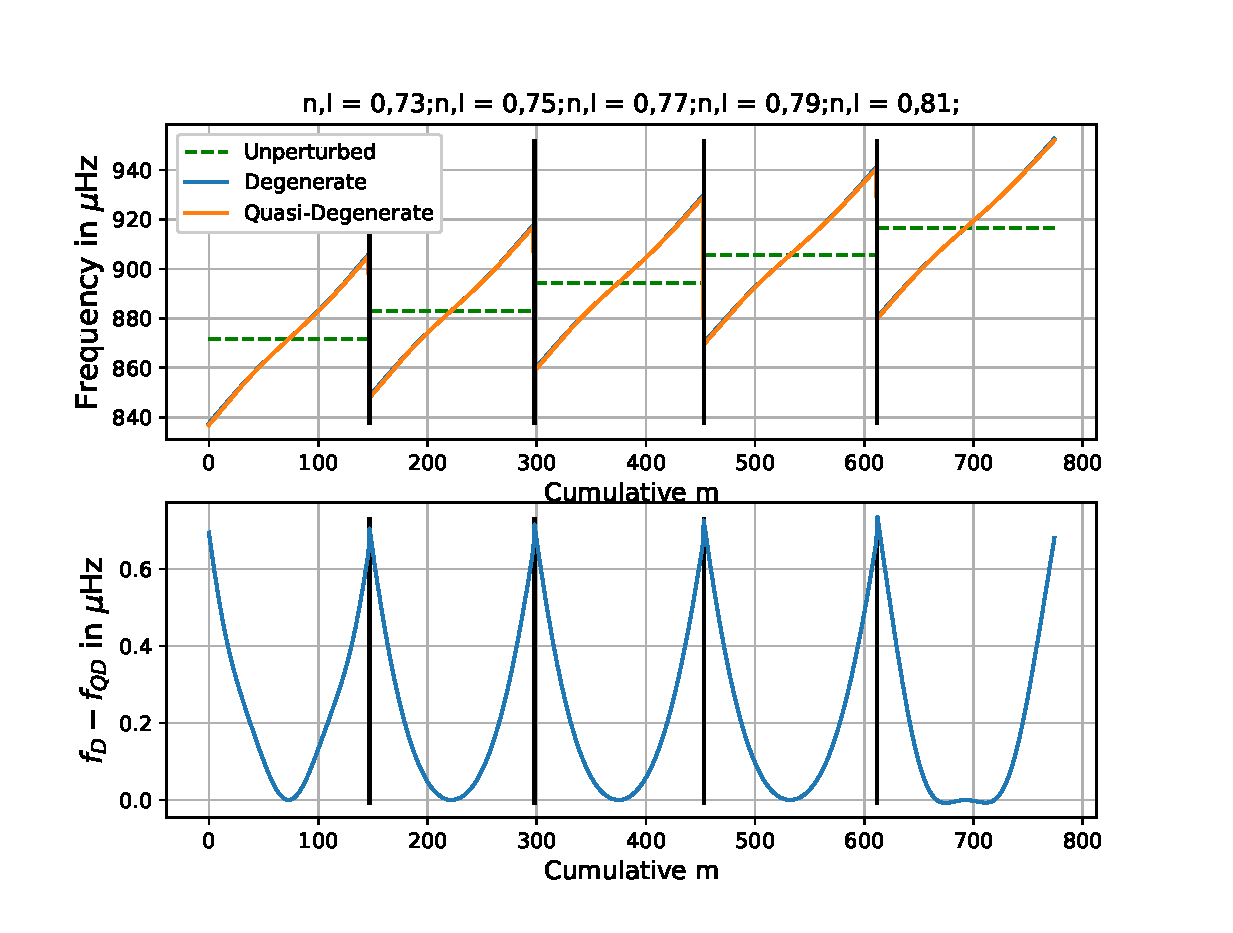
\includegraphics[scale=0.8,center]{Chapter4/figs/dr_split}
\caption{DPT and QDPT splits with $\mode{0}{73}$, $\mode{0}{75}$, $\mode{0}{77}$, $\mode{0}{79}$, and $\mode{0}{81}$ which have frequencies 871.63$\mu Hz$, 883.12$\mu Hz$, 894.43$\mu Hz$, 905.62$\mu Hz$, and 916.66$\mu Hz$ respectively. Top plot shows frequency splittings of the five modes and their unperturbed frequencies (green dashed). DPT and QDPT lie indiscernably   Bottom plot shows the departure of the DPT frequencies from the dpt frequencies.}
\label{fig:split_dr}
\end{figure}

$a$-coefficients obtained from the split is tabulated in table \ref{tab:split_dr}. $a_1$'s found from QDPT and DPT come out to be close to $440nHz$ which is corresponds to the $24$ day rotational cycle of the sun. $a_3$ and $a_5$ are found to be in good agreement upto a tolerance of $1nHz$. However, the QDPT profile contains even $a$-coefficients of the order of $5nHz$. This leads to an even profile departure of the QDPT from DPT profile of the order of $600nHz$ in the frequency spectrum as shown in figure (\ref{fig:split_dr}).

\begin{table}
\begin{center}
\begin{tabular}{|l|c|r|}
\hline
\textbf{Mode} & \textbf{QDPT(nHz)} & \textbf{DPT(nHz)} \\ \hline
$a_0$ &\hfill -2.832 & \hfill  - \\ \hline
$a_1$ & \hfill 438.378 & \hfill 438.178 \\ \hline
$a_2$ & \hfill -5.876 & \hfill - \\ \hline
$a_3$ & \hfill 22.149 & \hfill 22.005 \\ \hline
$a_4$ & \hfill -0.308 & \hfill  - \\ \hline
$a_5$ & \hfill -4.925 & \hfill -4.934 \\ \hline
$a_6$ & \hfill 0.091 & \hfill - \\ \hline
$a_7$ & \hfill -0.002 & \hfill  - \\ \hline
$a_8$ & \hfill -0.018 & \hfill - \\ \hline
$a_9$ & \hfill - & \hfill  - \\ \hline
$a_{10}$& \hfill  0.004 & \hfill  - \\ \hline
\end{tabular}
\end{center}
\caption{Splitting coefficients for mode $\mode{0}{77}$ via QDPT and DPT analysis. Hyphens stand for values $< 0.001nHz$.}
\label{tab:split_dr}
\end{table}

\subsection{Splitting with pure rotation removed}
We see that the component $w_1^0(r)$ in the sun's rotational profile gives rise to a velocity field
$$\mathbf{v} = -w_1^0 \partial_{\theta}Y_1^0 \ev{\phi} = \gam{1}w_1^0 \sin\theta \ev{\phi}$$
which corresponds to pure shell like rotation at each particular radius $r$. Taking $w_1^0 \rightarrow w_1^0 - \Omega_1 r / \gam{1}$ gives
\begin{equation}
\mathbf{v} = \gam{1}w_1^0 \sin\theta \ev{\phi} - \Omega_1 r \sin\theta \ev{\phi}
\end{equation}
and hence corresponds to slowing down each shell by an angular velocity $\Omega_1$ about the spin axis. Thus, subtracting out $\Omega_1 r / \gam{1}$ from $w_1^0$ is equivalent to slowing down the pure rotational profile by angular velocity $\Omega_1$.

We see that after removing an pure rotation component equivalent to 440nHz from the $w_1^0$ rotational profile, we get the following splitting of frequencies for QDPT and DPT respectively as shown in figure (\ref{fig:split_dr}). QDPT is performed taking 5 modes all lying in a band of width $100\mu Hz$.
\begin{figure}[h!]
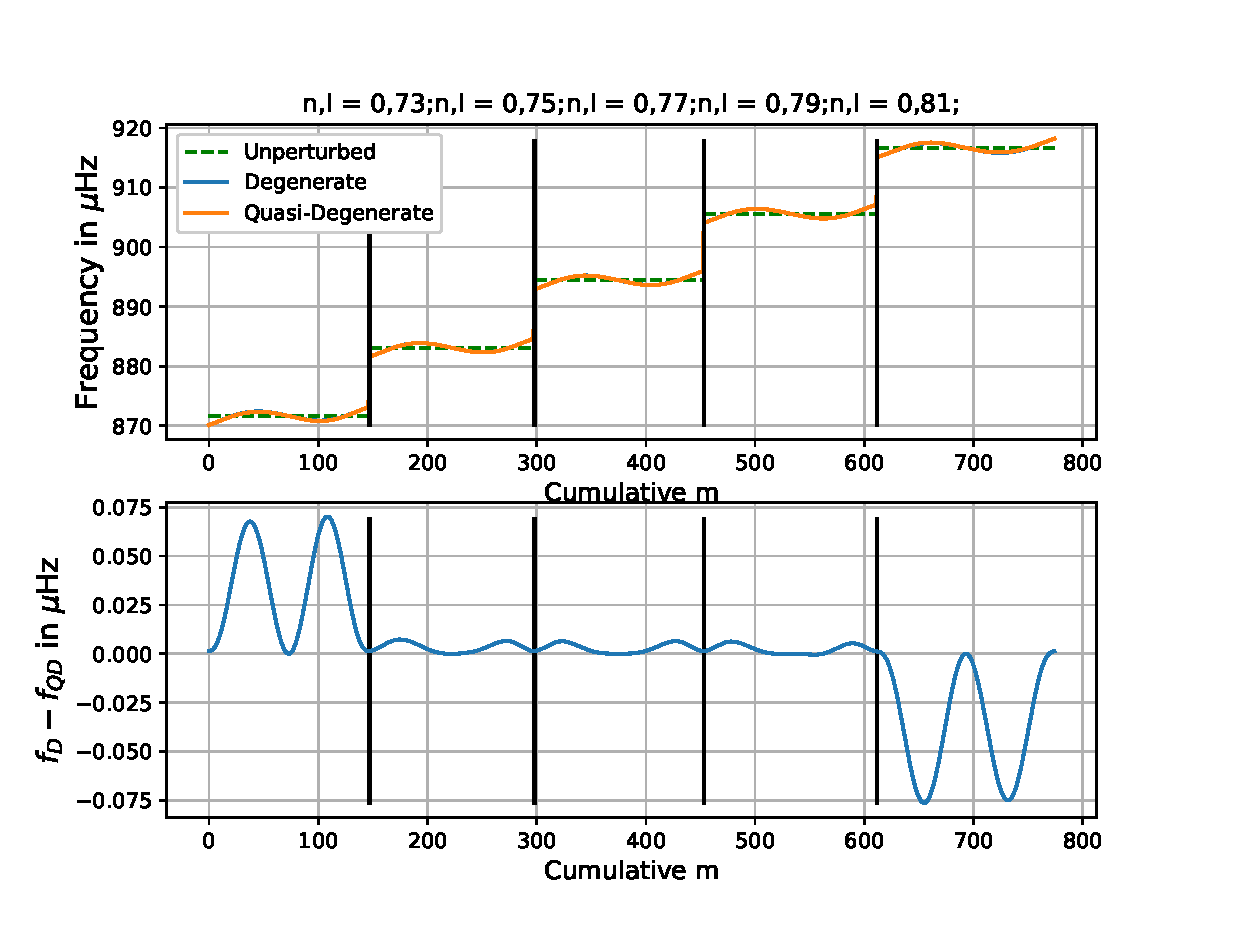
\includegraphics[scale=0.8,center]{Chapter4/figs/dr_split_rm}
\caption{DPT and QDPT rotational splits with pure rotational component equivalent to $440 nHz$ removed from $w_1^0$ for modes $\mode{0}{73}$, $\mode{0}{75}$, $\mode{0}{77}$, $\mode{0}{79}$, and $\mode{0}{81}$ which have frequencies as shown in table (\ref{tab:mode_list}). Top plot shows frequency splittings of the five modes and their unperturbed frequencies. Bottom plot shows the departure of the QDPT frequencies from the DPT frequencies.}
\label{fig:split_dr_rm}
\end{figure}

\begin{table}
\begin{center}
\begin{tabular}{|l|c|r|}
\hline
\textbf{Mode} & \textbf{QDPT(nHz)} & \textbf{DPT(nHz)} \\ \hline
$a_{0}$ & \hfill -0.038 &\hfill  - \\ \hline
$a_{1}$ & \hfill  2.820 &\hfill  2.820 \\ \hline
$a_{2}$ & \hfill -0.030 &\hfill - \\ \hline
$a_{3}$ & \hfill 22.005 &\hfill 22.005 \\ \hline
$a_{4}$ & \hfill  0.071 &\hfill  - \\ \hline
$a_{5}$ & \hfill -4.933 &\hfill -4.934 \\ \hline
$a_{6}$ & \hfill -0.006 &\hfill  - \\ \hline
$a_{7}$ & \hfill  - &\hfill  - \\ \hline
$a_{8}$ & \hfill -0.018 &\hfill - \\ \hline
$a_{9}$ & \hfill - &\hfill  - \\ \hline
$a_{10}$ & \hfill  0.004 &\hfill  - \\ \hline
\end{tabular}
\end{center}
\caption{Splitting coefficients for the splitting of mode $\mode{0}{77}$ by QDPT and DPT analysis after removing pure rotational component equivalent to $440nHz$ from $w_1^0$. Hyphens stand for values $< 0.001nHz$.}
\label{tab:split_dr_rm}
\end{table}

\subsubsection{QDPT vs DPT with increasing coupling modes}
When QDPT is performed taking multiple neighbouring modes amongst the ones in table \ref{tab:mode_list}, a peculiar trend is found when comparing QDPT frequencies with theri DPT counterparts for each singlet mode. The trend in figure (\ref{fig:DPT_err}) shows large deviations in QDPT splitting from from DPT frequencies in modes placed at either extreme regardless of how many modes couple while QDPT-DPT departure in the inner modes stay the same. This hints at the large QDPT-DPT frequency differences obtained for the extremal modes being artefacts of the calculation and hence being unreliable. For reference henceforth, we only use QDPT frequencies of $\mode{0}{77}$ which remains relatively unchanged with respect to number of modes being considered.

\begin{figure}[h]
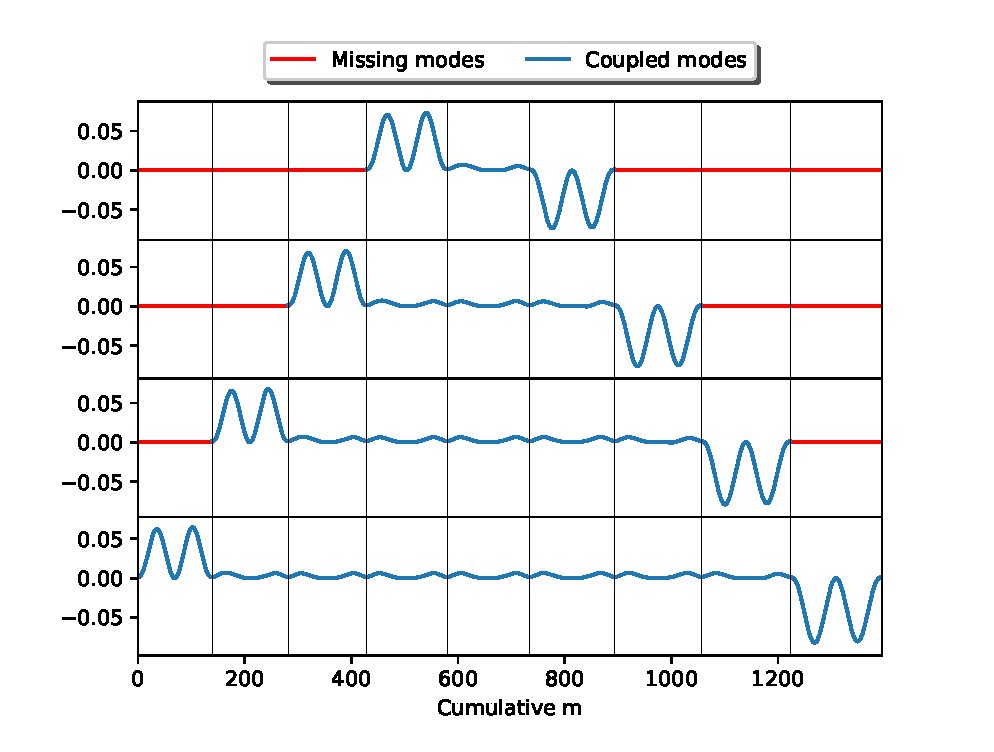
\includegraphics[scale=0.9, center]{Chapter4/figs/qdpt_err}
\caption{(QDPT - DPT) deviation with differing number of neighbouring modes being allowed to couple via differential rotation with mean rotation removed. From top, $\mode{0}{77}$ is made to couple with two, four, six, and eight closest $\Delta l=2$ neighbours (by frequency) as listed in table \ref{tab:mode_list}.}
\label{fig:DPT_err} 
\end{figure}

\section{Splittings due to Lorentz Stresses} %Section - 1.2

For finding magnetic splitting of the frequency spectrum, we choose to go to the corotating frame ($440 nHz$) to eliminate the dominant linear trend from the splitting profile and perform QDPT with the perturbation $\dLB$ on a background spectrum which is already split by differential rotation. We are justified in doing this because eliminating a net rotational component is equivalent to a coordinate transformation \cite{jcd_notes}. In this treatment where the background profile is already  split by differential rotation, our perturbation which couples different modes is $\dLB$ (equation  (\ref{eqn:dLB})). Background frequencies $\omega_{nlm}$ are obtained by performing DPT on degenerate modes $\mode{n}{l}$. We have chosen to perform DPT over QDPT for obtaining background $\omega_{nlm}$'s to reduce computational burden because resultant frequencies differ by less than $10nHz$ (centre section of figure (\ref{fig:split_dr_rm}) corresponding to $\mode{0}{77}$) and odd $a$-coefficients are almost identical (table \ref{tab:split_dr} shows the low relative error in odd $a$-coefficients).

The departure from the (rotating) background of the spectrum is shown in figure (\ref{fig:mag_split}). The $a$-coefficients are listed in table \ref{tab:mag_split}. The table also contains the $a$-coefficients for magnetic splitting obtained from QDPT performed on a background with no rotation for comparison.

\begin{figure}[h!]
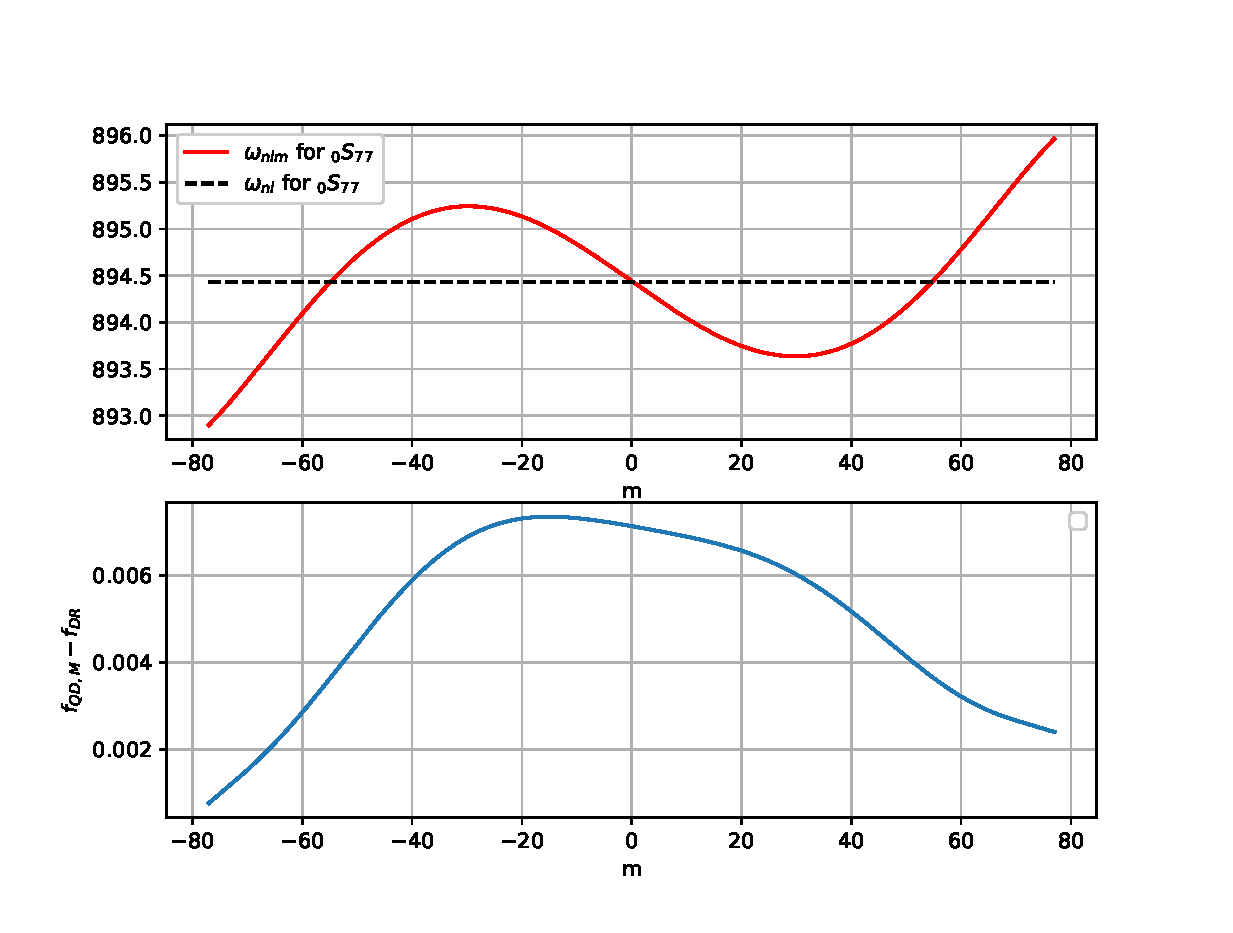
\includegraphics[scale=0.9, center]{Chapter4/figs/mag_split}
\caption{Magnetic splitting profile of the mode \mode{0}{77} obtained from QDPT containing all nine modes listed in table \ref{tab:mode_list} on rotating background with $440nHz$ equivalent component removed from $w_1^0$. Top shows the absolute frequency about the unperturbed baseline in $\mu HZ$. Bottom shows the difference between the overall (rotation + magnetic field) and the background rotation profile obtained from DPT.}
\label{fig:mag_split}
\end{figure}

\subsection{Detectibility}
the first two columns of table \ref{tab:mag_split} show the effect of magnetic perturbation on even $a$-coefficients. While the non-magnetic rotating profile (obatined by DPT) contains no evn $a$'s at all, the magnetic perturbation introduces $a_0=63 pHz$ and $a_2=-59pHz$. These $pHz$ level $a$-coefficients are not detectable by current standards of precision in observation as minimum errors in observed coefficients lie in the $\sim 1nHz$ range \cite{schou_data}.

\begin{table}
\begin{center}
\begin{tabular}{|l|c|c|r|}
\hline
\textbf{$\bm{a}_n$} & \shortstack{\textbf{Magnetic QDPT} \\ \textbf{(on rotating} \\ \textbf{ background)}} & \shortstack{\textbf{Rotating} \\ \textbf{ Background} \\ \textbf{(no magnetic field)}} & \shortstack{\textbf{Magnetic DPT} \\ \textbf{(on stationary} \\ \textbf{ background)}} \\ \hline
$a_{0}$ & \hfill  0.063 & \hfill - & \hfill  0.061 \\ \hline
$a_{1}$ & \hfill  2.822 & \hfill  2.820 &\hfill  - \\ \hline
$a_{2}$ & \hfill -0.059 & \hfill - & \hfill -0.059 \\ \hline
$a_{3}$ & \hfill 22.020 & \hfill 22.005 & \hfill  - \\ \hline
$a_{4}$ & \hfill -  &\hfill  -&\hfill - \\ \hline
$a_{5}$ & \hfill -4.937 &\hfill -4.934 &\hfill  - \\ \hline
%$a_{6}$ & \hfill - &\hfill  - \\ \hline
%$a_{7}$ & \hfill  - &\hfill - \\ \hline
%$a_{8}$ & \hfill - &\hfill  - \\ \hline
%$a_{9}$ & \hfill - &\hfill  - \\ \hline
%$a_{10}$ & \hfill - &\hfill  - \\ \hline
\end{tabular}
\end{center}
\caption{Splitting coefficients in $nHz$ for the magnetic splitting of mode $\mode{0}{77}$. First column is magnetic QDPT split on differentially rotating background (pure rotation removed) obtained by DPT. Second column in the background split for the first column. Third column is magnetic DPT performed on stationary sun. List has been truncated whence $a$'s vanish identically. Hyphens stand for values $< 0.001nHz$.}
\label{tab:mag_split}
\end{table}

\section{Conclusion}

We had started out with the goal of solving the forward problem of finding splittings in degenerate modes in the sun's acoustic frequency spectrum. This was aimed at the possibility of a future project to image the interior magnetic field by performing an inversion procedure on the observed splitting data by using the Lorentz stress sensitivity kernels obtained in \ref{sec:mag_kern}. We constructed a magnetic field profile closely mimicking that of the sun to validate the kernels found. We found, by feeding our synthetic magnetic field in the sensitivity kernels and performing QDPT on nine neighbouring modes, that additional components of about $60pHz$ to $a_0$ and $a_2$ coefficients are being introduced to the splitting of the mode $\mode{0}{77}$. These changes to $a$-coefficients are smaller than errors in $a$-coefficients to have been recorded till now, and hence not detectable with current levels of available precision. In future, an increase in precision of recording these coefficients by two orders of magnitude will enable a realistic inversion of splitting data aimed at imaging Lorentz stress components in the interior of the sun.

